\documentclass[tikz]{standalone}
\usepackage{tikz}
\usepackage{pgfplots}
\usepackage{ifthen}
\usetikzlibrary{arrows.meta,positioning,fit,calc,shapes.geometric,shapes.symbols,shapes.multipart,backgrounds,matrix}
\pgfplotsset{compat=1.18}

\definecolor{medblue}{RGB}{34,91,169}
\definecolor{medcyan}{RGB}{25,166,200}
\definecolor{medgreen}{RGB}{64,142,86}
\definecolor{medgold}{RGB}{207,157,41}
\definecolor{medred}{RGB}{176,64,64}
\definecolor{medgray}{RGB}{79,88,102}
\definecolor{medlight}{RGB}{245,247,250}
\definecolor{gold}{RGB}{207,157,41}

\tikzset{
base/.style={draw=medgray, rounded corners=3pt, very thick, align=center, inner sep=7pt, fill=white, font=\fontsize{10}{12}\selectfont},
service/.style={base, fill=blue!7, draw=medblue, minimum width=3.1cm, minimum height=1.15cm},
store/.style={base, fill=green!8, draw=medgreen, minimum width=2.8cm, minimum height=1.05cm},
actor/.style={base, fill=gold!10, draw=medgold, minimum width=2.4cm, minimum height=1cm},
process/.style={base, fill=cyan!10, draw=medcyan, minimum width=2.8cm, minimum height=1.05cm},
external/.style={base, fill=red!8, draw=medred, minimum width=2.8cm, minimum height=1.05cm},
arrow/.style={-{Latex[length=3mm,width=2mm]}, very thick, draw=medgray},
biarrow/.style={{Latex[length=3mm,width=2mm]}-{Latex[length=3mm,width=2mm]}, very thick, draw=medgray},
note/.style={align=left, font=\fontsize{10}{12}\selectfont, text=medgray},
titlebox/.style={draw=medblue, fill=medlight, rounded corners=4pt, inner sep=5pt, font=\fontsize{11}{13}\selectfont\bfseries},
group/.style={draw=medgray!70, dashed, rounded corners=6pt, inner sep=8pt}
}
\begin{document}
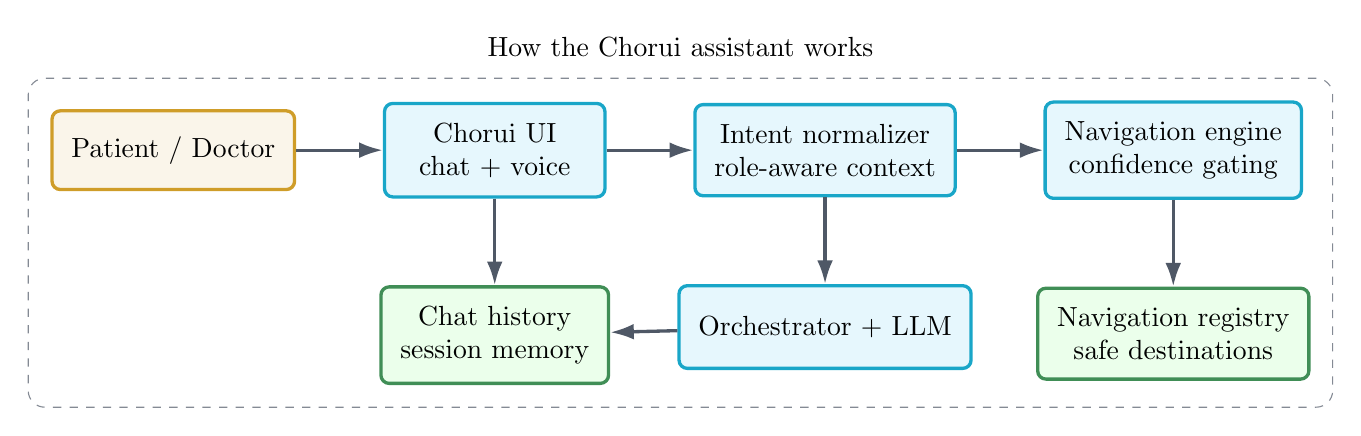
\begin{tikzpicture}[node distance=1.1cm and 1.1cm]
\node[actor] (user) {Patient / Doctor};
\node[process, right=of user] (ui) {Chorui UI\\chat + voice};
\node[process, right=of ui] (intent) {Intent normalizer\\role-aware context};
\node[process, right=of intent] (nav) {Navigation engine\\confidence gating};
\node[process, below=of intent] (llm) {Orchestrator + LLM};
\node[store, below=of nav] (registry) {Navigation registry\\safe destinations};
\node[store, below=of ui] (history) {Chat history\\session memory};
\draw[arrow] (user) -- (ui);
\draw[arrow] (ui) -- (intent);
\draw[arrow] (intent) -- (nav);
\draw[arrow] (intent) -- (llm);
\draw[arrow] (nav) -- (registry);
\draw[arrow] (ui) -- (history);
\draw[arrow] (llm) -- (history);
\node[group, fit=(user)(ui)(intent)(nav)(llm)(registry)(history), label={[yshift=0.15cm]above:How the Chorui assistant works}] {};
\end{tikzpicture}
\end{document}